\documentclass[11pt,a4paper]{article}

\usepackage[utf8]{inputenc}
\usepackage[T1]{fontenc}
\usepackage{amsmath,amssymb}
\usepackage{graphicx}
\usepackage{booktabs}
\usepackage{hyperref}
\usepackage{float}
\usepackage[margin=1in]{geometry}
\usepackage{caption}
\usepackage{enumitem}

\hypersetup{colorlinks=true, linkcolor=blue, citecolor=blue, urlcolor=blue}

\newcommand{\R}{\mathbb{R}}
\DeclareMathOperator*{\argmin}{argmin}
\DeclareMathOperator{\FFT}{FFT}
\DeclareMathOperator{\PSD}{PSD}

\title{Linear Decoding Reveals a Shared Manifold\\Between Language and Time Series Representations}
\author{Prateek Humane}
\date{}

\begin{document}
\maketitle

\begin{abstract}
Why can language models be finetuned to forecast time series?
We present evidence for a \textit{shared manifold hypothesis}: autoregressive pretraining compresses hidden state trajectories onto a low-dimensional manifold whose geometry is naturally compatible with real-world temporal data.
To test this, we train a single linear projection to decode time series from the hidden states of a pretrained Qwen3-0.6B model processing WikiText---with no paired text--time-series supervision and no model finetuning.
The decoded outputs closely match real time series from GiftEval, producing 686 unique matches across 14 of 20 temporal clusters.
A $2\times 2$ ablation crossing \textit{architecture} (pretrained vs.\ random weights) with \textit{input} (text vs.\ random tokens) confirms that this alignment requires both components: pretraining creates the shared manifold, and meaningful text drives diverse traversal of it.
PCA analysis reveals the manifold's structure: pretrained representations occupy a $\sim$6-dimensional subspace of the full 28{,}672-dimensional space, with 80\% of variance in a single direction.
This shared low-dimensional geometry---smooth, low-frequency, temporally coherent---explains both why language-to-time-series transfer works and why it succeeds through linear probing alone.
\end{abstract}

% ──────────────────────────────────────────────────────────────
\section{Introduction}

Language models pretrained on text can be finetuned to forecast time series, often matching or outperforming domain-specific architectures. This surprising cross-modal transfer raises a fundamental question: \textit{why should representations learned from text be useful for temporal data?}

We propose the \textbf{shared manifold hypothesis}: autoregressive pretraining compresses hidden state trajectories onto a low-dimensional manifold whose geometry is inherently compatible with time series data. The mechanism is intuitive. When a transformer processes a sequence of tokens, each layer produces a hidden state that evolves smoothly from one position to the next---each transformer layer applies a residual update, so $\mathbf{h}_{t+1} \approx \mathbf{h}_t + \delta_t$, producing trajectories that are smooth, temporally coherent, and low-frequency dominated. These are precisely the statistical properties that characterize real-world time series: trends, level shifts, and slowly-varying periodicity. Pretraining does not teach the model about time series explicitly; rather, it compresses text representations onto a manifold whose temporal dynamics \textit{happen to share geometric structure} with temporal data.

To test this, we attempt the most direct possible experiment: take a pretrained language model processing ordinary Wikipedia text and ask whether a single linear projection of its hidden states---trained without any paired text--time-series data and without finetuning the model---can produce realistic time series. The fact that this works provides direct evidence that language models and time series occupy a shared representational manifold.

% ──────────────────────────────────────────────────────────────
\section{Setup and Method}

\paragraph{Models.} Qwen3-0.6B (28 layers, $d{=}1024$) in two variants: \textbf{PT} (pretrained) and \textbf{RandomInit} (random weights, same architecture).

\paragraph{Data.} \textit{Text}: WikiText-103 ($N{=}1920$ train, $1000$ held-out sequences of $T{=}512$ tokens). \textit{Time series}: 10{,}000 z-normalized windows ($T{=}512$) from GiftEval. \textit{Random tokens}: uniformly sampled from the full vocabulary ($|\mathcal{V}|{=}151{,}936$).

\paragraph{Hidden states.} We concatenate all 28 layer outputs per timestep:
$\mathbf{h}_{i,t} = [\mathbf{h}_{i,t}^{(0)}; \ldots; \mathbf{h}_{i,t}^{(27)}] \in \R^{D}$, $D = 28{,}672$.

\paragraph{Linear decoding.} A per-timestep linear map $\hat{y}_{i,t} = \mathbf{w}^\top \mathbf{h}_{i,t} + b$ produces a predicted sequence $\hat{\mathbf{y}}_i \in \R^T$, z-normalized to zero mean and unit variance. This is a single direction in hidden state space---if that direction aligns with time-series-like dynamics, the output will resemble real temporal data.

\paragraph{Training.} Since we have no paired supervision, we train via EM-style nearest-neighbor matching: each predicted sequence is matched to its closest real time series, and the map is optimized to minimize MSE to these assignments. A spectral diversity penalty prevents collapse:
\begin{equation}
    \mathcal{L} = \underbrace{\tfrac{1}{B}\textstyle\sum_i \tfrac{1}{T}\|\hat{\mathbf{y}}_i - \mathbf{Y}_{j_i^*}\|^2}_{\text{MSE to nearest real TS}} + \;\lambda \underbrace{\tfrac{1}{|\mathcal{P}|}\textstyle\sum_{(i,j)\in\mathcal{P}} \cos\!\bigl(|\FFT(\hat{\mathbf{y}}_i)|^2,\, |\FFT(\hat{\mathbf{y}}_j)|^2\bigr)}_{\text{penalize spectral similarity in batch}}
\end{equation}
where $j_i^* = \argmin_j \|\hat{\mathbf{y}}_i - \mathbf{Y}_j\|^2$ (with stop-gradient) and $\lambda = 0.5$.

\begin{figure}[t]
\centering
\includegraphics[width=\textwidth]{figures/fig_text_pt_examples.png}
\caption{Time series linearly decoded from WikiText hidden states (blue) overlaid with their nearest real time series from GiftEval (green), at quality ranks \#1 through \#100. No text--time-series pairing was used during training. The decoded signals capture trends, level shifts, and oscillatory structure present in the real data.}
\label{fig:examples}
\end{figure}

% ──────────────────────────────────────────────────────────────
\section{The $2\times 2$ Ablation}

The text + PT result could be driven by three distinct factors: the \textit{architecture} (transformer inductive biases), the \textit{learned weights} (what pretraining encodes), or the \textit{data} (structure in natural text). Our $2 \times 2$ ablation disentangles these by independently varying the model (PT vs.\ RandomInit, same architecture) and the input (text vs.\ random tokens). Comparing PT to RandomInit isolates the effect of learned weights while holding architecture fixed. Comparing text to random tokens isolates the effect of input structure while holding the model fixed.

\begin{table}[h]
\centering
\begin{tabular}{lrrrrr}
\toprule
Condition & Train Unique & Held-Out Unique & Train NN & Held-Out NN & Clusters \\
\midrule
\textbf{text + PT} & \textbf{686}/1920 & \textbf{439}/1000 & 0.672 & 0.717 & 14/20 \\
text + RandInit & 54/1920 & 73/1000 & 0.402 & 0.541 & 13/20 \\
rand + PT & 4/1920 & 1/1000 & 0.283 & 0.293 & 4/20 \\
rand + RandInit & 99/1920 & 138/1000 & 0.522 & 0.741 & 14/20 \\
\bottomrule
\end{tabular}
\caption{$2\times 2$ ablation. \textit{Unique}: distinct real TS matched out of the total predictions (which are matched against a bank of 10{,}000 real TS). \textit{NN}: mean nearest-neighbor MSE (low NN with low Unique = mode collapse, not quality). \textit{Clusters}: ACF-based cluster coverage.}
\label{tab:ablation}
\end{table}

The results decompose cleanly:

\paragraph{text + PT (686 unique).} The only condition that produces diverse, high-quality outputs. Pretrained representations encode smooth temporal structure; meaningful text drives the hidden state along varied trajectories through this structured space; the linear map projects these trajectories into time-series-like signals. The mapper generalizes to held-out text (439 unique on unseen WikiText), confirming the alignment is not memorized.

\paragraph{rand + PT (4 unique).} Pretrained weights still create low-dimensional structure, but random tokens fail to \textit{traverse} it. The model maps all random inputs to a narrow region of representation space, so the linear map---no matter how well-trained---produces near-identical outputs. The structure exists but is not activated.

\paragraph{text + RandInit (54 unique).} Text varies but the random model cannot transform that variation into structured representations. Without pretraining, hidden states are high-dimensional noise---there is no low-dimensional manifold for a linear map to exploit.

\paragraph{rand + RandInit (99 unique $>$ 54).} Random tokens through random weights slightly outperform text through random weights. This confirms the RandInit model does not ``understand'' text: it treats all inputs as arbitrary vectors, so higher input entropy (random tokens span the full vocabulary) directly translates to more output diversity.

\paragraph{Fair quality comparison.} Raw NN distance is misleading---rand + PT's 0.283 reflects 4 repeated matches, not quality. Comparing at matched diversity:

\begin{table}[h]
\centering
\begin{tabular}{rcccc}
\toprule
$K$ & text + PT & text + RandInit & rand + PT & rand + RandInit \\
\midrule
4 & \textbf{0.254} & 0.383 & 0.330 & 0.412 \\
99 & \textbf{0.383} & 0.825 & --- & 0.862 \\
200 & \textbf{0.441} & 0.971 & --- & 1.004 \\
\bottomrule
\end{tabular}
\caption{Top-$K$ fair comparison: mean NN distance of the best-$K$ unique matches. text + PT produces both more \textit{and} better-quality matches at every $K$.}
\label{tab:topk}
\end{table}

% ──────────────────────────────────────────────────────────────
\section{Evidence for the Shared Manifold}

The ablation shows \textit{that} pretraining is necessary. We now ask \textit{why}---and find the answer in the geometry of the representation space itself.

\subsection{The manifold is low-dimensional}

PCA on flattened hidden states ($50{,}000$ random samples from the $N{\times}T{\times}D$ tensor per condition) reveals a stark geometric contrast.

\begin{table}[h]
\centering
\begin{tabular}{lrrrr}
\toprule
Condition & Eff.\ Rank & Top Eigenvalue & Mean Var & PCs for 90\% \\
\midrule
text + PT & 5.6 & 81.5\% & 104.4 & 60 \\
rand + PT & 2.8 & 89.2\% & 93.1 & 2 \\
text + RandInit & 431 & 3.0\% & 3.8 & 421 \\
rand + RandInit & 585 & 1.7\% & 3.9 & 500+ \\
\bottomrule
\end{tabular}
\caption{Representation geometry. Effective rank $= \exp(-\sum p_i \log p_i)$ where $p_i = \lambda_i / \mathrm{Tr}(\Sigma)$. Pretraining compresses 28{,}672 dimensions into $\sim$3--6 effective dimensions. Random initialization yields near-isotropic geometry.}
\label{tab:pca}
\end{table}

Pretrained models concentrate $>$80\% of variance into a single principal direction, yielding effective ranks of 3--6. Random models spread variance across 400--600 directions with no dominant component.

\subsection{Why the manifold aligns with time series}

The key insight is that a low-dimensional representation with smooth temporal evolution \textit{is} a time series. The shared manifold arises not from any explicit connection between language and temporal data, but from the dynamics of autoregressive processing. Consider what happens as a language model processes a 512-token text sequence:

\begin{enumerate}[nosep]
    \item The hidden state $\mathbf{h}_t$ evolves gradually from one token to the next---each transformer layer applies a residual update, so $\mathbf{h}_{t+1} \approx \mathbf{h}_t + \delta_t$ where $\delta_t$ is typically small relative to $\mathbf{h}_t$.
    \item Pretraining compresses these trajectories onto a low-dimensional manifold: despite $D = 28{,}672$ dimensions, the hidden states effectively occupy a $\sim$6-dimensional subspace.
    \item Any linear projection of a smooth, low-dimensional trajectory produces a smooth, one-dimensional signal---exactly the kind of slowly-varying, low-frequency-dominated pattern that characterizes real time series.
\end{enumerate}

This is why the alignment is \textit{geometric}, not semantic. The decoded time series do not ``mean'' anything related to the input text. Rather, the \textit{shape} of activation trajectories in a pretrained transformer---smooth, low-rank, temporally coherent---happens to occupy the same statistical space as real temporal data.

\subsection{Spectral evidence}

This geometric account predicts that decoded outputs should be low-frequency dominated, like real time series. We confirm this by comparing power spectral density:

\begin{center}
\small
\begin{tabular}{lrrr}
\toprule
& Low freq (0--10\%) & Mid (10--50\%) & High (50--100\%) \\
\midrule
text + PT & 90.1\% & 6.6\% & 3.3\% \\
text + RandInit & 58.4\% & 19.5\% & 22.1\% \\
Real TS & 79.2\% & 13.7\% & 7.2\% \\
\bottomrule
\end{tabular}
\end{center}

PT outputs concentrate 90\% of energy in the lowest 10\% of frequencies, closely matching the 79\% of real time series. RandInit outputs are spectrally flat (58\% low, 22\% high)---consistent with projecting isotropic, high-dimensional noise rather than structured low-dimensional trajectories.

\begin{figure}[t]
\centering
\includegraphics[width=\textwidth]{figures/fig_pca_spectrum.png}
\caption{PCA eigenvalue spectrum (top 100 components). PT models (blue, green) show extreme concentration: the first eigenvalue dwarfs all others. RandInit models (orange, pink) show flat spectra with no dominant direction. This anisotropy is why linear decoding finds signal in pretrained representations but not in random ones.}
\label{fig:pca}
\end{figure}

\begin{figure}[t]
\centering
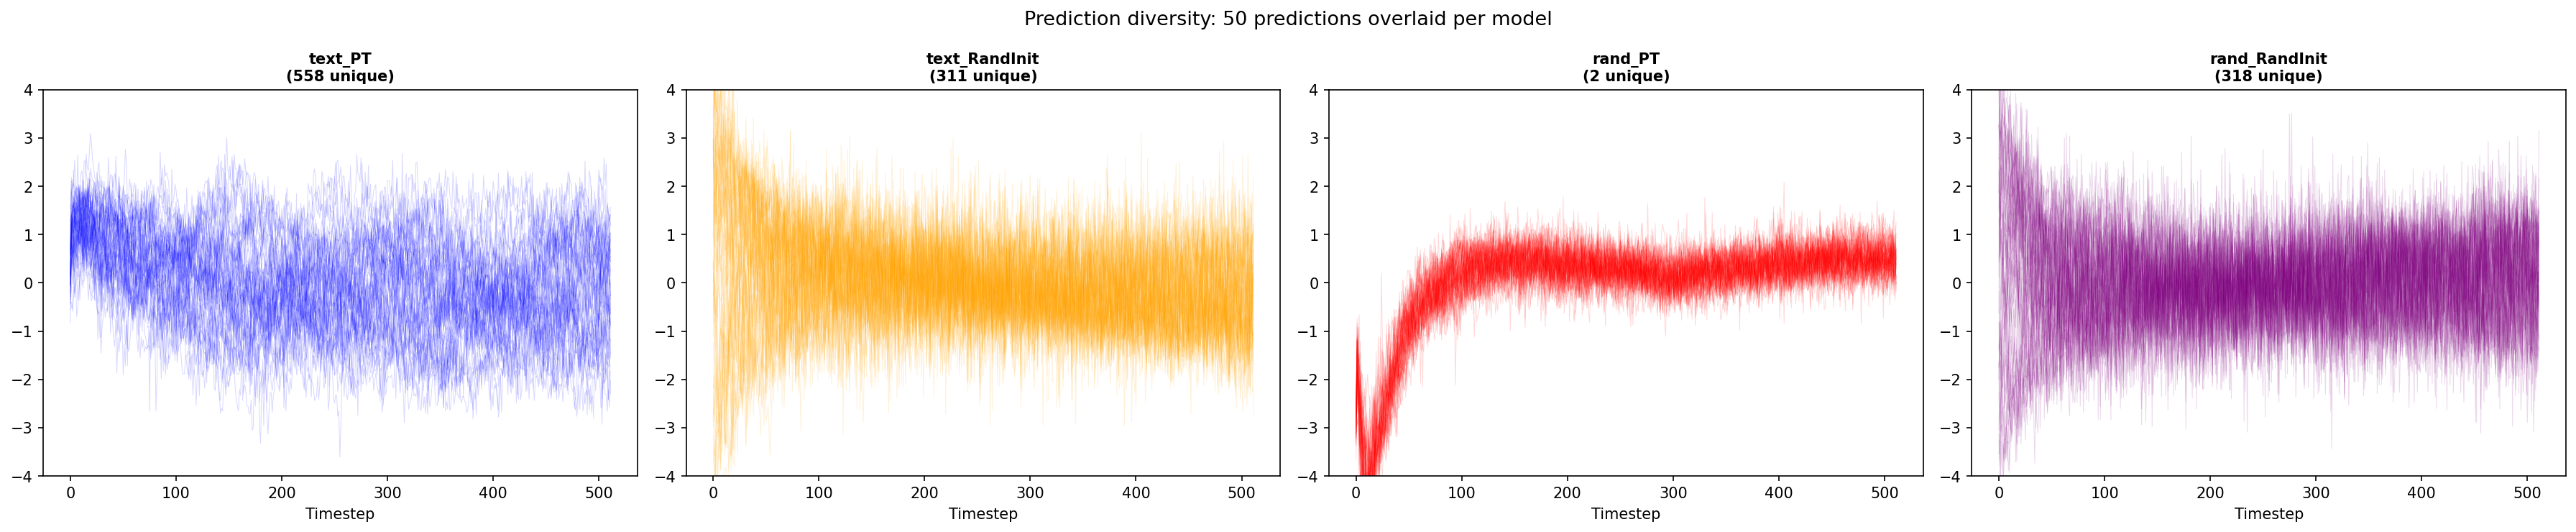
\includegraphics[width=\textwidth]{figures/fig_diversity.png}
\caption{50 random decoded sequences per condition. text + PT (top-left) produces diverse waveforms spanning trends, oscillations, and level shifts. rand + PT (bottom-left) collapses to a single repeated shape---the manifold exists but isn't traversed. RandInit conditions (right) produce noisy, structureless variation.}
\label{fig:diversity}
\end{figure}

% ──────────────────────────────────────────────────────────────
\section{Conclusion}

We have presented evidence for a shared manifold hypothesis: pretrained language models and real-world time series occupy a common low-dimensional subspace in representation space. A single linear projection decodes realistic time series from WikiText hidden states without paired supervision or model finetuning. The $2 \times 2$ ablation confirms this requires pretrained weights (which create the manifold) \textit{and} meaningful text (which traverses it). PCA reveals the manifold's extreme compactness: effective rank $\sim$6 in 28{,}672 dimensions, with 80\% of variance in one direction.

The shared manifold arises because autoregressive pretraining compresses sequential representations into smooth, low-frequency trajectories---the same temporal statistics that dominate real-world time series. This geometric alignment explains why language models transfer so effectively to time series tasks.

However, the connection may go deeper than pure geometry. Concurrent crosscoder analysis on the same model reveals that individual neural features activated by semantically temporal language---words like \textit{slope}, \textit{rise}, \textit{decline}, \textit{steady}---also fire on corresponding time series patterns when the model is finetuned on temporal data. If single tokens can activate representations that capture local temporal structure (a rise, a plateau, a sharp drop), then a \textit{sequence} of such tokens---an ordinary sentence whose meaning unfolds over time---would trace a trajectory through activation space that naturally assembles into a full time series window. The shared manifold, in this view, is not merely a statistical coincidence but a reflection of the fact that language \textit{about} temporal phenomena and temporal phenomena \textit{themselves} are encoded by overlapping neural circuits. The linear map we train may simply be recovering this alignment.

\end{document}
